\documentclass[]{beamer}
\usepackage{tikz,lstautogobble,listings}
\usetikzlibrary{arrows.meta}
\usetheme{Rochester}
\usepackage[T1]{fontenc}
\usepackage[utf8]{inputenc}
\usetikzlibrary{arrows.meta}
\lstset{
  language=caml,
  basicstyle=\ttfamily\tiny,
  breaklines=true,
  autogobble=true,
}


\title{TIPE 25/26 - Cycles et Boucles}
\author{GIL Dorian}
\subtitle{Une étude de la Méthode des tableaux}
\date{}

\begin{document}

\begin{frame}
\titlepage
\end{frame}

\begin{frame}
    \begin{itemize}
        \item Une étude en logique propositionelle
        \item Une étude en logique linéaire temporelle
    \end{itemize}
\end{frame}
\begin{frame}{Position du problème}
    \begin{itemize}[<+->]
        \item On cherche à étudier une méthode algorithmique permettant de montrer la satisfiabilité d'une formule: la Méthode des tableaux.
        \item Cette méthode consiste à construire un arbre avec la formule à la racine, et à utiliser des règles pour développer ou créer des branches.
        \item On regarde ensuite si il y a des contradictions dans toutes les branches, si c'est le cas, la formule est insatisfaisable.
        \item Cette méthode est utilisé dans diverses logiques, pour l'instant, on se restreint à la logique propositionnelle.
    \end{itemize}
\end{frame}

\begin{frame}{Un exemple graphique}
    \textbf{Formule:} $\lnot(a \Rightarrow (b \Rightarrow a))$

    \begin{center}
        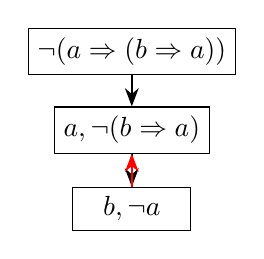
\begin{tikzpicture}[
            every node/.style={draw, minimum width=1.5cm, align=center},
            every arrow/.style={thick,->,>=Stealth}
        ]
        \node (root) at (0,0) {$\lnot(a \Rightarrow (b \Rightarrow a))$};
        \pause
        \node (not_b_a) at (0,-1) {$a, \lnot(b \Rightarrow a)$};
        \draw[every arrow] (root) -- (not_b_a);
        \pause
        \node (b) at (0,-2) {$b, \lnot a$};
        \draw[every arrow] (not_b_a) -- (b);
        \pause
        \draw[red,every arrow] (b) -- (not_b_a);
        \end{tikzpicture}
    \end{center}
\end{frame}

\begin{frame}{Petite étude introductive}
    Après l'avoir implémenter, j'ai décidé de me resteindre à une forme particulière de formule logique.
    \begin{definition}[Forme Alternée]
        Soit $n\in\mathbb{N}^*$, et $(a_k)_{k\in [|1,n|]}$ des litteraux, on dit que $\varphi$ est de forme alternée ssi
        $$\varphi = a_1\land(a_2\lor(a_3\land(\dots(a_n))))$$
    \end{definition}
    Notre but en faisant une restriction du problème est:
    \begin{itemize}
        \item De mieux comprendre les avantages de cette méthode (dans quelle type de formule la méthode est-elle meilleur ?)
        \item De trouver des algorithmes polynomiales pour nos restrictions (si ce n'est possible, alors on améliorera aux maximum l'algorithme)
    \end{itemize}
\end{frame}

\begin{frame}{Une reécriture}
    En utilisant une propriété que j'ai démontré, on va re-écrire l'arbre induit par la méthode des tableaux d'une manière différente:
    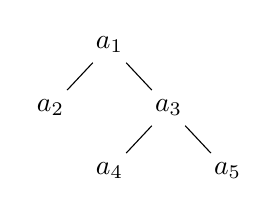
\begin{tikzpicture}[level distance=8mm]
        \node {$a_1$}
            child {node {$a_2$}}
            child {node {$a_3$}
            child {node {$a_4$}}
            child {node {$a_5$}}};
    \end{tikzpicture}

    Au lieu de :

    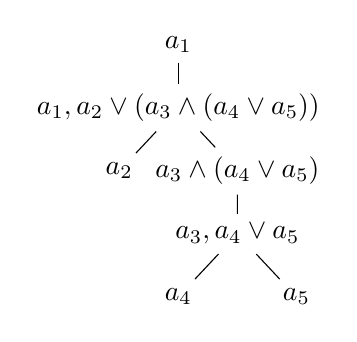
\begin{tikzpicture}[level distance=8mm]
        \node {$a_1$}
            child {node {$a_1 , a_2\lor(a_3\land(a_4\lor a_5))$}
                child {node {$a_2$}}
                child {node {$a_3\land(a_4\lor a_5)$}
                    child {node {$a_3 , a_4\lor a_5$}
                        child {node {$a_4$}}
                        child {node {$a_5$}}
                        }
                }
            };
    \end{tikzpicture}
    Pour $\varphi = a_1\land(a_2\lor(a_3\land(a_4\lor a_5)))$
\end{frame}

\begin{frame}{Résolution du problème}
    L'algorithme récursif consiste à faire ces analyses (en créant un dictionnaire stockant le "signe" des litteraux):
    \begin{enumerate}
        \item On analyse le litteral droit, si il y a contradiction, l'arbre est fermé, sinon on ajoute eventuellement dans le dictionnaire le litteral
        \item On analyse le litteral gauche, si il produit une contradiction, appel recursif plus profond dans l'arbre, sinon la formule est satisfiable
    \end{enumerate}
    Le cas de base étant l'arrivée au bout du peigne.
    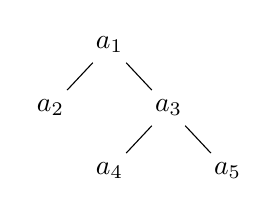
\begin{tikzpicture}[level distance=8mm]
        \node {$a_1$}
            child {node {$a_2$}}
            child {node {$a_3$}
            child {node {$a_4$}}
            child {node {$a_5$}}};
    \end{tikzpicture}
\end{frame}

\begin{frame}{Preuves et stats}
    L'algorithme est en $\mathcal{O}(n)$, en supposant les opérations Hashtbl constantes.
    \pause
    \begin{itemize}
        \item La correction (preuve faite) est assuré par l'invariant "Toutes les branches déjà traités sont fermés"
        \item La terminaison (preuve faite) est assuré simplement.
    \end{itemize}
    \pause
    On créé une base de donnée de 100 formules de forme alternée et on fait tourner Quine et notre algorithme dessus.
    \begin{itemize}
        \item \textbf{Alternée:} 0.000493s
        \item \textbf{Quine (avec conversion en CNF):} 0.025874s
        \item \textbf{Quine (sans conversion en CNF):} 0.018691s
    \end{itemize} 
\end{frame}
 
\begin{frame}{Conclusion}
    Bien entendu, il n'est pas possible de convertir toutes les formules en Alternée.

    On a donc trouvé un exemple de type de formule qui est facile à analyser par méthode des tableaux.
\end{frame}

\begin{frame}{Introduction à la LTL 1}
    \begin{definition}[Formule de la LTL]
        On définit $F$ l'ensemble des formules de la LTL inductivement par:
        \begin{itemize}
            \item $p\in AP \implies p\in F$
            \item si $\psi$ et $\phi$ sont des formules de LTL alors $\lnot\psi, \phi\lor\psi, X\psi, \phi U\psi$ sont des formules de LTL
        \end{itemize}
        $AP$ un ensemble fini de variables propositionnelles.
    \end{definition}
    \begin{definition}[Opérateurs X et U]
        On les définit par:
            \begin{itemize}
                \item $X\phi$ : $\phi$ doit être satisfaite dans l'état suivant (neXt)
                \item $\psi U\phi$ : $\psi$ doit être satisfaite dans tous les états jusqu'à un état où $\phi$ est satisfait (Until)
            \end{itemize}
    \end{definition}
\end{frame}

\begin{frame}{Introduction à la LTL 2}
     \begin{definition}[Monde]
        On définit un tel objet comme $\omega := w_0,w_1,\dots$ une suite infinie d'état.
        On écrira $\omega^i:=w_i,w_{i+1},\dots$ un suffixe de $\omega$.
    \end{definition}
    Soit $v : \omega\times F \rightarrow \{T,F\}$ une fonction de valuation.
    \begin{definition}[Satisfaction d'un monde]
        En LTL, on définit $\omega \models f$ via:
        \begin{itemize}
            \item $\omega \models a \Leftrightarrow v(w_0,a) = T$ si $a$ atomique 
            \item $\omega \models \lnot f$ si $\lnot(\omega \models f)$ 
            \item $\omega \models f\lor g$ si $\omega \models f$ ou $\omega \models g$
            \item $\omega \models \textbf{X}f$ si $\omega^1 \models f$
            \item $\omega \models f\textbf{U}g$ si $\omega \models g$ ou $\omega \models f\land\textbf{X}(f\textbf{U}g)$
        \end{itemize}
    \end{definition}
\end{frame}

\begin{frame}{Introduction à la LTL 3}
    On peut trouver plusieurs applications à la LTL:
    \begin{itemize}
        \item Preuve de programme concurrentiel
        \item Raisonnement sur des circuits intégrés
        \item Raisonnement sur les protocoles de communications
    \end{itemize}
    Toutes ces applications s'inscrivent dans le cadre de la vérification de modèles qui est une méthode permettant de montrer
    la correction de systèmes informatiques complexes.

    \begin{definition}[Verification de modèle (Model Checking)]
        Technique de vérification qui explore tout les états possible d'un système de manière force brute.
    \end{definition}
\end{frame}

\begin{frame}{Model Checking}
    Ici, nous nous interesserons pas aux techniques utilisés dans le domaine.
    On retiendra seulement que la méthode des tableaux est très utilisé dans la logique modale qui englobe la LTL et que
    elle est particulièrement utile pour certaines techniques de vérifications de modèles.

    Ainsi, nous allons étudier un exemple de formule de la LTL et étudier sa résolution par méthode des tableaux.
\end{frame}

\begin{frame}{Méthode des tableaux}
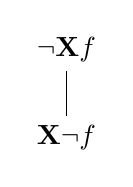
\begin{tikzpicture}[scale=0.75]
    \node {$\lnot\textbf{X}f$}
        child {node {$\textbf{X}\lnot f$}};
    \end{tikzpicture}
    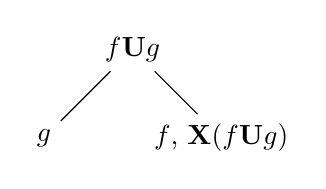
\begin{tikzpicture}[scale=0.75, level 1/.style={sibling distance=3cm}]
    \node {$f\textbf{U}g$}
        child {node {$g$}}
        child{node {$f$, $\textbf{X}(f\textbf{U}g)$}};
    \end{tikzpicture}
    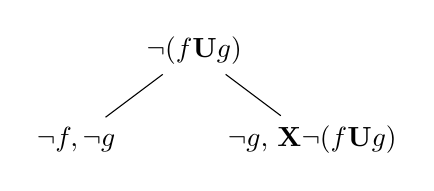
\begin{tikzpicture}[scale=0.75, level 1/.style={sibling distance=4cm}]
    \node {$\lnot(f\textbf{U}g)$}
        child {node {$\lnot f, \lnot g$}}
        child{node {$\lnot g$, $\textbf{X}\lnot(f\textbf{U}g)$}};
    \end{tikzpicture}

    \begin{definition}[Formule élementaire]
        $f$ est élementaire ssi il respecte un de ses 2 points:
        \begin{itemize}
            \item C'est une formule atomique (ou la négation d'une formule atomique)
            \item Il a comme connecteur logique "principale" $\textbf{X}$ (des X-formules)
        \end{itemize}
    \end{definition}
    Si un noeud contient uniquement des formules elementaires, alors on créé un fils
    du noeud contenant toutes les \textbf{X}-formules sans leur connecteur logique principal $\textbf{X}$

    A REVOIR
\end{frame}

\begin{frame}[fragile]{Code - Méthode des tableaux classique 1}
    \begin{center}
        \begin{tabular}{c}
            \begin{lstlisting}
                type prop = | Var of string | Not of prop | And of prop * prop | Or  of prop * prop
                (* Une branche c'est une liste de formule avec un signe *)
                type branch =  (bool * prop) list

                let is_literal = function
                    | (true, Var _) -> true
                    | (false, Var _) -> true
                    | (true, Not (Var _)) -> true
                    | (false, Not (Var _)) -> true
                    | _ -> false
            
                (* Check les contradictions *)
                let branch_closed (br : branch) : bool =
                    let pos = Hashtbl.create 16 in
                    let neg = Hashtbl.create 16 in
                    let record = function
                        | (true, Var v) -> Hashtbl.replace pos v true
                        | (false, Var v) -> Hashtbl.replace neg v true
                        | (true, Not (Var v)) -> Hashtbl.replace neg v true
                        | (false, Not (Var v)) -> Hashtbl.replace pos v true
                        | _ -> ()
                    in
                    List.iter record br;
                    let closed = ref false in
                    Hashtbl.iter (fun v _ -> if (Hashtbl.mem pos v) && (Hashtbl.mem neg v) then closed := true) pos;
                    !closed
            \end{lstlisting}
        \end{tabular}
      \end{center}
\end{frame}

\begin{frame}[fragile]{Code - Méthode des tableaux classique 2}
    \begin{center}
        \begin{tabular}{c}
            \begin{lstlisting}
            (* La decomposition usuelle faites durant la methode des tableaux *)
            let decompose_once (br : branch) : branch list option =
                let rec find_nonlit acc = function
                    | [] -> None
                    | x :: xs ->
                    if is_literal x then find_nonlit (x::acc) xs
                    else Some (List.rev acc, x, xs)
                in
                match find_nonlit [] br with
                | None -> None
                | Some (left, (sign, form), right) ->
                    let rest = left @ right in
                    let mk b p = (b, p) in
                    (match sign, form with
                    | true, And (a,b) ->
                    Some [ (mk true a) :: (mk true b) :: rest ]
                    | false, Or (a,b) ->
                    Some [ (mk false a) :: (mk false b) :: rest ]
                    | true, Or (a,b) ->
                    Some [ (mk true a)::rest; (mk true b)::rest ]
                    | false, And (a,b) ->
                    Some [ (mk false a)::rest; (mk false b)::rest ]
                    | true, Not a ->
                    Some [ (mk false a) :: rest ]
                    | false, Not a ->
                    Some [ (mk true a) :: rest ]
                    | _, _ -> None)
            \end{lstlisting}
        \end{tabular}
    \end{center}
\end{frame}


\begin{frame}[fragile]{Code - Méthode des tableaux classique 3}
    \begin{center}
        \begin{tabular}{c}
            \begin{lstlisting}
                (* La Methode des Tableaux en soit *)
                let satisfiable (phi : prop) : bool =
                let initial_branch = [ (true, phi) ] in
                let rec explore_stack stack =
                    match stack with
                    | [] -> false
                    | br :: rest ->
                    if branch_closed br then explore_stack rest else
                    match decompose_once br with
                    | None -> true
                    | Some new_branches -> explore_stack (new_branches @ rest)
                    in explore_stack [ initial_branch ]
            \end{lstlisting}
        \end{tabular}
    \end{center}
\end{frame}

\begin{frame}[fragile]{Code - Alternée 1}
    \begin{center}
        \begin{tabular}{c}
            \begin{lstlisting}
                type formula =
                    | Atom of (string* bool)
                    | And of (string*bool) * formula
                    | Or of (string*bool) * formula

                type branch = 
                    | Empty
                    | Node of (formula option * formula * branch);;

                let extract (f:formula option) = match f with
                    | None ->  Atom("none", false)
                    | Some t -> t

                let rec print_formula (f:formula) = match f with
                    | Atom(s, b) -> if b then print_string s else print_string "Not ";print_string s;
                    | And ((f, b),g) -> if b then print_string f else print_string "Not ";print_string f;print_string " And ";print_formula g
                    | Or ((f,b),g) -> if b then print_string f else print_string "Not ";print_string f;print_string " Or ";print_formula g;;

                let rec print_branches (b:branch) =
                    print_string " [";
                    match b with
                        | Empty -> ()
                        | Node(a1, a2, b) -> print_formula@@extract a1;print_string ", ";print_formula a2;print_branches b;
                    print_string "]";; 
            \end{lstlisting}
        \end{tabular}
    \end{center}   
\end{frame}

\begin{frame}[fragile]{Code - Alternée 2}
    \begin{center}
        \begin{tabular}{c}
            \begin{lstlisting}
            let rec formula2branch (f:formula) : branch = match f with
                | And(a, Or(b, Atom(c))) -> Node(Some(Atom b), Atom a, Node(None, Atom(c), Empty))
                | And(a, Or(b, c)) ->  Node(Some(Atom b), Atom a, formula2branch c)
                | And(a, Atom(b)) -> Node(Some (Atom b), Atom a, Empty)
                | _ -> failwith "Pas alternee"
              
            let has_cycle (br:branch) : bool = 
                let rec aux (br:branch) (d:(string,bool) Hashtbl.t) : bool = match br with
                | Node(None, Atom (f, b), Empty) -> 
                  if Hashtbl.mem d f then 
                    Hashtbl.find d f = b
                  else
                    true
                | Node(Some(Atom(fg, bg)), Atom (fd, bd), Empty) -> 
                      if Hashtbl.mem d fd then
                        if Hashtbl.find d fd = bd then
                          not @@ Hashtbl.mem d fg && Hashtbl.find d fg <> bg
                        else 
                          false
                      else(
                        Hashtbl.add d fd bd;
                        not @@ Hashtbl.mem d fg && Hashtbl.find d fg <> bg)
                | Node(Some (Atom (fg, bg)), Atom (fd, bd), nb) ->
                  if Hashtbl.mem d fd then
                    if Hashtbl.find d fd <> bd then
            \end{lstlisting}
        \end{tabular}
    \end{center}   
\end{frame}

\begin{frame}[fragile]{Code - Alternée 3}
    \begin{center}
        \begin{tabular}{c}
            \begin{lstlisting}
                        false
                            else
                            if Hashtbl.mem d fg then
                                if Hashtbl.find d fg = bg then
                                true
                                else
                                aux nb d
                            else
                                true
                        else
                            (Hashtbl.add d fd bd;
                            if Hashtbl.mem d fg then
                            if Hashtbl.find d fg = bg then
                                true
                            else
                                aux nb d
                            else
                            true)
                        | _ -> failwith "Pas alternee"
                        in aux br (Hashtbl.create 100);;
          
                        let is_satisfiable (f:formula) : bool = let b = formula2branch f in has_cycle b;;
            \end{lstlisting}
        \end{tabular}
    \end{center}   
\end{frame}
\end{document}